\subsection[Satz von Ladner]{Satz von Ladner}

\begin{frame}
	Frage : Gibt es $\NP$  Probleme , die nicht \NP -vollständig sind , aber auch nicht in $\P$  liegen
\end{frame}
\begin{frame}
	\begin{figure} 
		%\centering 
		\caption[NP-Intermediate]{$\NP$-Intermediate} 
		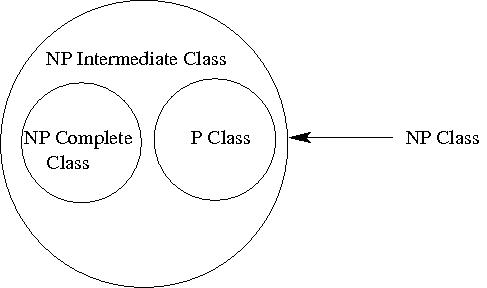
\includegraphics[scale = 0.4]{images/np-intermediate} 
		\newline 
		\label[http://functionspace.org/articles/28/Complexity-Zoo] 
	\end{figure}
\end{frame}
\begin{frame}
	Mögliche Kandidaten :
	\begin{itemize}
	\item Graphisomorphie (kommt in Vortrag 7)
	\item Faktorisierungsproblem
	\item Kein "natürlicher" Kandidat bekannt
	\end{itemize}
	
	aber,
\end{frame}

\begin{frame}
	\begin{Satz}[Existenz einer \NP -intermediate Sprache, Ladner, 75]
	Wenn $\P \neq \NP$ dann gilt : \newline
	Es existiert eine Sprache $L \in \NP \setminus \P$ die nicht \NP -vollständig ist
	\end{Satz}
\end{frame}